%!TEX root = ../hbrs-poster.tex


    \block{Abstract}
    {
        % \begin{wrapfigure}{l}{16cm}
        %     \vspace{-1cm}
        %     \begin{tikzfigure}
        %         
\includegraphics[scale=0.225]{figures/b-it.pdf}
        %     \end{tikzfigure}
        % \end{wrapfigure}
        Online platforms increasingly rely on automated systems to moderate content and ensure respectful discourse. Identifying toxic comments is crucial for maintaining community standards and protecting users from harmful interactions. We are using the dataset from the "Toxic Comment Classification Challenge" \cite{jigsaw-toxic-comment-classification-challenge} on Kaggle that provides a benchmark dataset \cite{kaggle_toxic} for developing models that can classify online comments into multiple toxicity categories, such as threats, obscenity, or hate speech. We explored different NLP techniques for multi-class classification and investigated how different architectures and embeddings influence classification performance. We found that Transformers (BERT, T5, GPT-1, etc) outperform traditional NLP approaches such as SVM, XGBoost, etc. Our dataset was an unbalanced dataset, the distribution of which you can find in the plot below.

            \begin{center}
                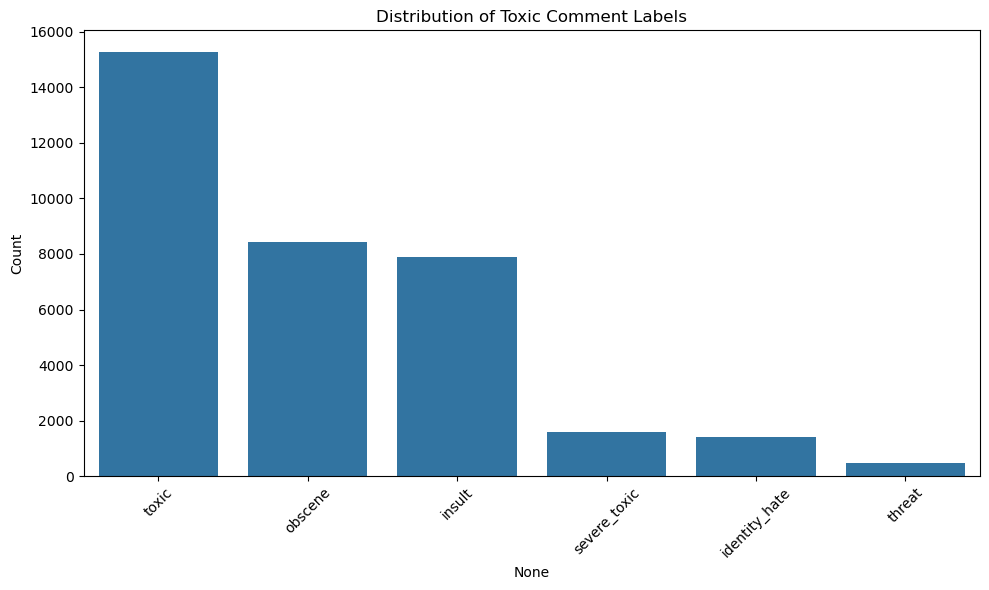
\includegraphics[width=0.3\textwidth]{figures/dataset_distribution.png}
                \captionof{figure}{Distribution of the dataset used for toxic comment classification}
                \label{fig:dataset-distribution}
            \end{center}
    }

